%%%%%%%%%%%%%%%%%%%%%%%%%%%%%%%%%%%%%%%
\section{Il modello di adronizzazione statistica}
I \emph{modelli di adronizzazione statistica} (SHM), chiamati anche modelli termici-statistici, sono utilizzati per predire l'abbondanza delle diverse specie di particelle prodotte nelle collisioni di particelle.
Questi modelli assumono che le particelle vengano emesse da una sorgente in equilibrio termico e chimico e che ogni tipo di particella abbia la possibilità di essere prodotta, purché vengano rispettate le leggi di conservazione previste dal Modello Standard.
Le abbondanze relative delle specie che vengono prodotte tuttavia verranno regolate dalle leggi della meccanica statistica, in particolare dipenderanno fortemente dalla funzione di partizione, la quale a sua volta dipenderà dal mezzo in cui avviene la collisione.
Il mezzo che si considera in questo caso è quello di un gas in espansione, non interagente, composto da particelle e risonanze, che chiamiamo \emph{Gas di Risonanze Adroniche} (HRG).
A seconda del sistema  considerato abbiamo due casi principali: se il volume di interazione è sufficientemente grande (per esempio nelle collisioni di ioni pesanti) si utilizza allora il modello statistico con un ensemble gran canonico; mentre se il volume è ridotto allora si utilizza il modello statistico nell'ensemble canonico.\\

Nel formalismo dell'ensemble gran canonico si prevede un sistema che interagisce con un reservoir, scambiando con esso energia e particelle.
Il sistema che si considera in questo caso è la regione misurabile dai rilevatori di ALICE, in contatto con il reservoir che si forma quando vi è una collisione di ioni pesanti, ossia l'HRG (non il Quark-Gluon Plasma perché esso non è invece accessibile dai rilevatori).
Assumendo che vi sia un equilibrio tra la regione e il reservoir, allora ciò implica una conservazione in media dell'energia e delle principali grandezze quantistiche, come la carica e i numeri quantici.
Quindi si utilizza il formalismo gran canonico per ottenere le proprietà statistiche di questi sistemi fisici.
Per far ciò si utilizza la funzione di partizione $Z$ e sapendo che dipende da queste proprietà, possiamo assumere che $Z = Z(T,V,\mu)$, con $T$ la temperatura del mezzo, $V$ il volume, $\mu$ il potenziale chimico collettivo definito come $\mu = \sum_iQ_i\mu_i$, con $\mu_i$ i potenziali chimici relativi a ogni carica conservata $Q_i$.
Nel reservoir, le principali grandezze che vengono conservate sono la carica elettrica $Q$, la stranezza $S$ e il numero barionico $B$.
La funzione gran canonica, data la non-interazione tra le particelle, può essere considerata come prodotto delle funzioni di partizione di singolo stato di particella,
\begin{gather}
    Z(T,V,\mu) = \prod_i Z_i(T,V,\mu_i)\\
    \implies \log Z(T,V,\mu)= \sum_i \log Z_i(T,V,\mu_i)
\end{gather}
Si può dimostrare che la funzione che descrive $\log Z_i$ ha la seguente espressione
\begin{equation}
    \log Z_i(T,V,\mu_i) = \dfrac{Vg_i}{2\pi\beta\pi^2}\sum_{k=1}^\infty \dfrac{(\pm 1)^{k+1}}{k^2}\lambda_i^k m_i^2 \ K_2(k\beta m_i) 
\end{equation}
con $g_i$ la molteplicità spin-isospin della particella nello stato $i$, $m_i$ è la sua massa, $K_2$ la funzione modificata di Bessel del secondo tipo; il termine $\pm$ assume valore $+1$ per particelle descritte dalla statistica di Bose-Einstein e $-1$ per le particelle descritte dalla statistica di Fermi-Dirac.
Una quantità interessante da ricavare è il numero medio di particelle di uno stato $i$, ottenibile da
\begin{equation}\label{eq:mean_n}
    \lrangle{N_i}_\text{th}(T,V,\mu) = \dfrac1\beta\pd{}{\mu_i} \log Z_i(T,V,\mu_i)
\end{equation}
Tuttavia questa descrizione è incompleta dal momento in cui non si è tenuto conto di contributi da parte degli stati di risonanza.
Facendo così si ottiene il numero medio totale di particelle dello stato $i$ come
\begin{equation}
    \lrangle{N_i}_\text{tot}(T,V,\mu) = \lrangle{N_i}_\text{th}(T,V,\mu) + \sum_j \Gamma_{j\to i}\lrangle{N_i}_\text{th}(T,V,\mu)
\end{equation}
con $\Gamma_{j\to i}$ il coefficiente del contributo della risonanza $j$ che decade in $i$.
Quindi il numero medio delle particelle dipende principalmente da cinque parametri, ossia la temperatura, il volume e i tre potenziali chimici.\\

Il modello di adronizzazione statistica canonica (CSM) invece riguarda volumi di interazioni minori ottenuti per esempio in collisioni pp.
Essendo il volume di interazione ridotto, allora la conservazione delle cariche non può essere più assunta in media, ma deve essere esatta, ossia senza fluttuazioni.
Questo significa che il numero di particelle cariche è soppresso rispetto a quello del modello gran canonico, per questo viene dato il nome di \emph{soppressione canonica}.
La trattazione del modello canonico è simile a quello gran canonico: si assume il HRG in equilibrio termico come sistema, caratterizzato da un volume e temperatura, con le cariche conservate ($Q$, $B$ e $S$).
Un fattore aggiuntivo da tenere in considerazione rispetto alla trattazione gran canonica in questo caso è il \emph{fattore chimico}, il quale assicura la conservazione della carica locale.
Uno degli effetti della soppressione canonica è la riduzione della produzione delle particelle con stranezza.\\

\subsection{Predizioni del SHM}
Tramite il modello SHM sono possibili diverse predizioni:
\begin{itemize}
    \item predizioni della produzione di adroni dotati di una massa variabile in una vasto intervallo di valori, si parla da pioni fino ai (anti)nuclei come l'$^{4}{\rm He}$.
    In \autoref{fig:mass_yield} si può osservare che il modello è preciso nella predizione per i nuclei, mentre tende a sottostimare leggermente la produzione degli adroni più leggeri se non si considera il contributo dovuto ai decadimenti degli stati risonanti.
    Questi non contribuiscono significativamente alla produzione di particelle massive come i nuclei.
\begin{figure}[htpb]
    \centering
    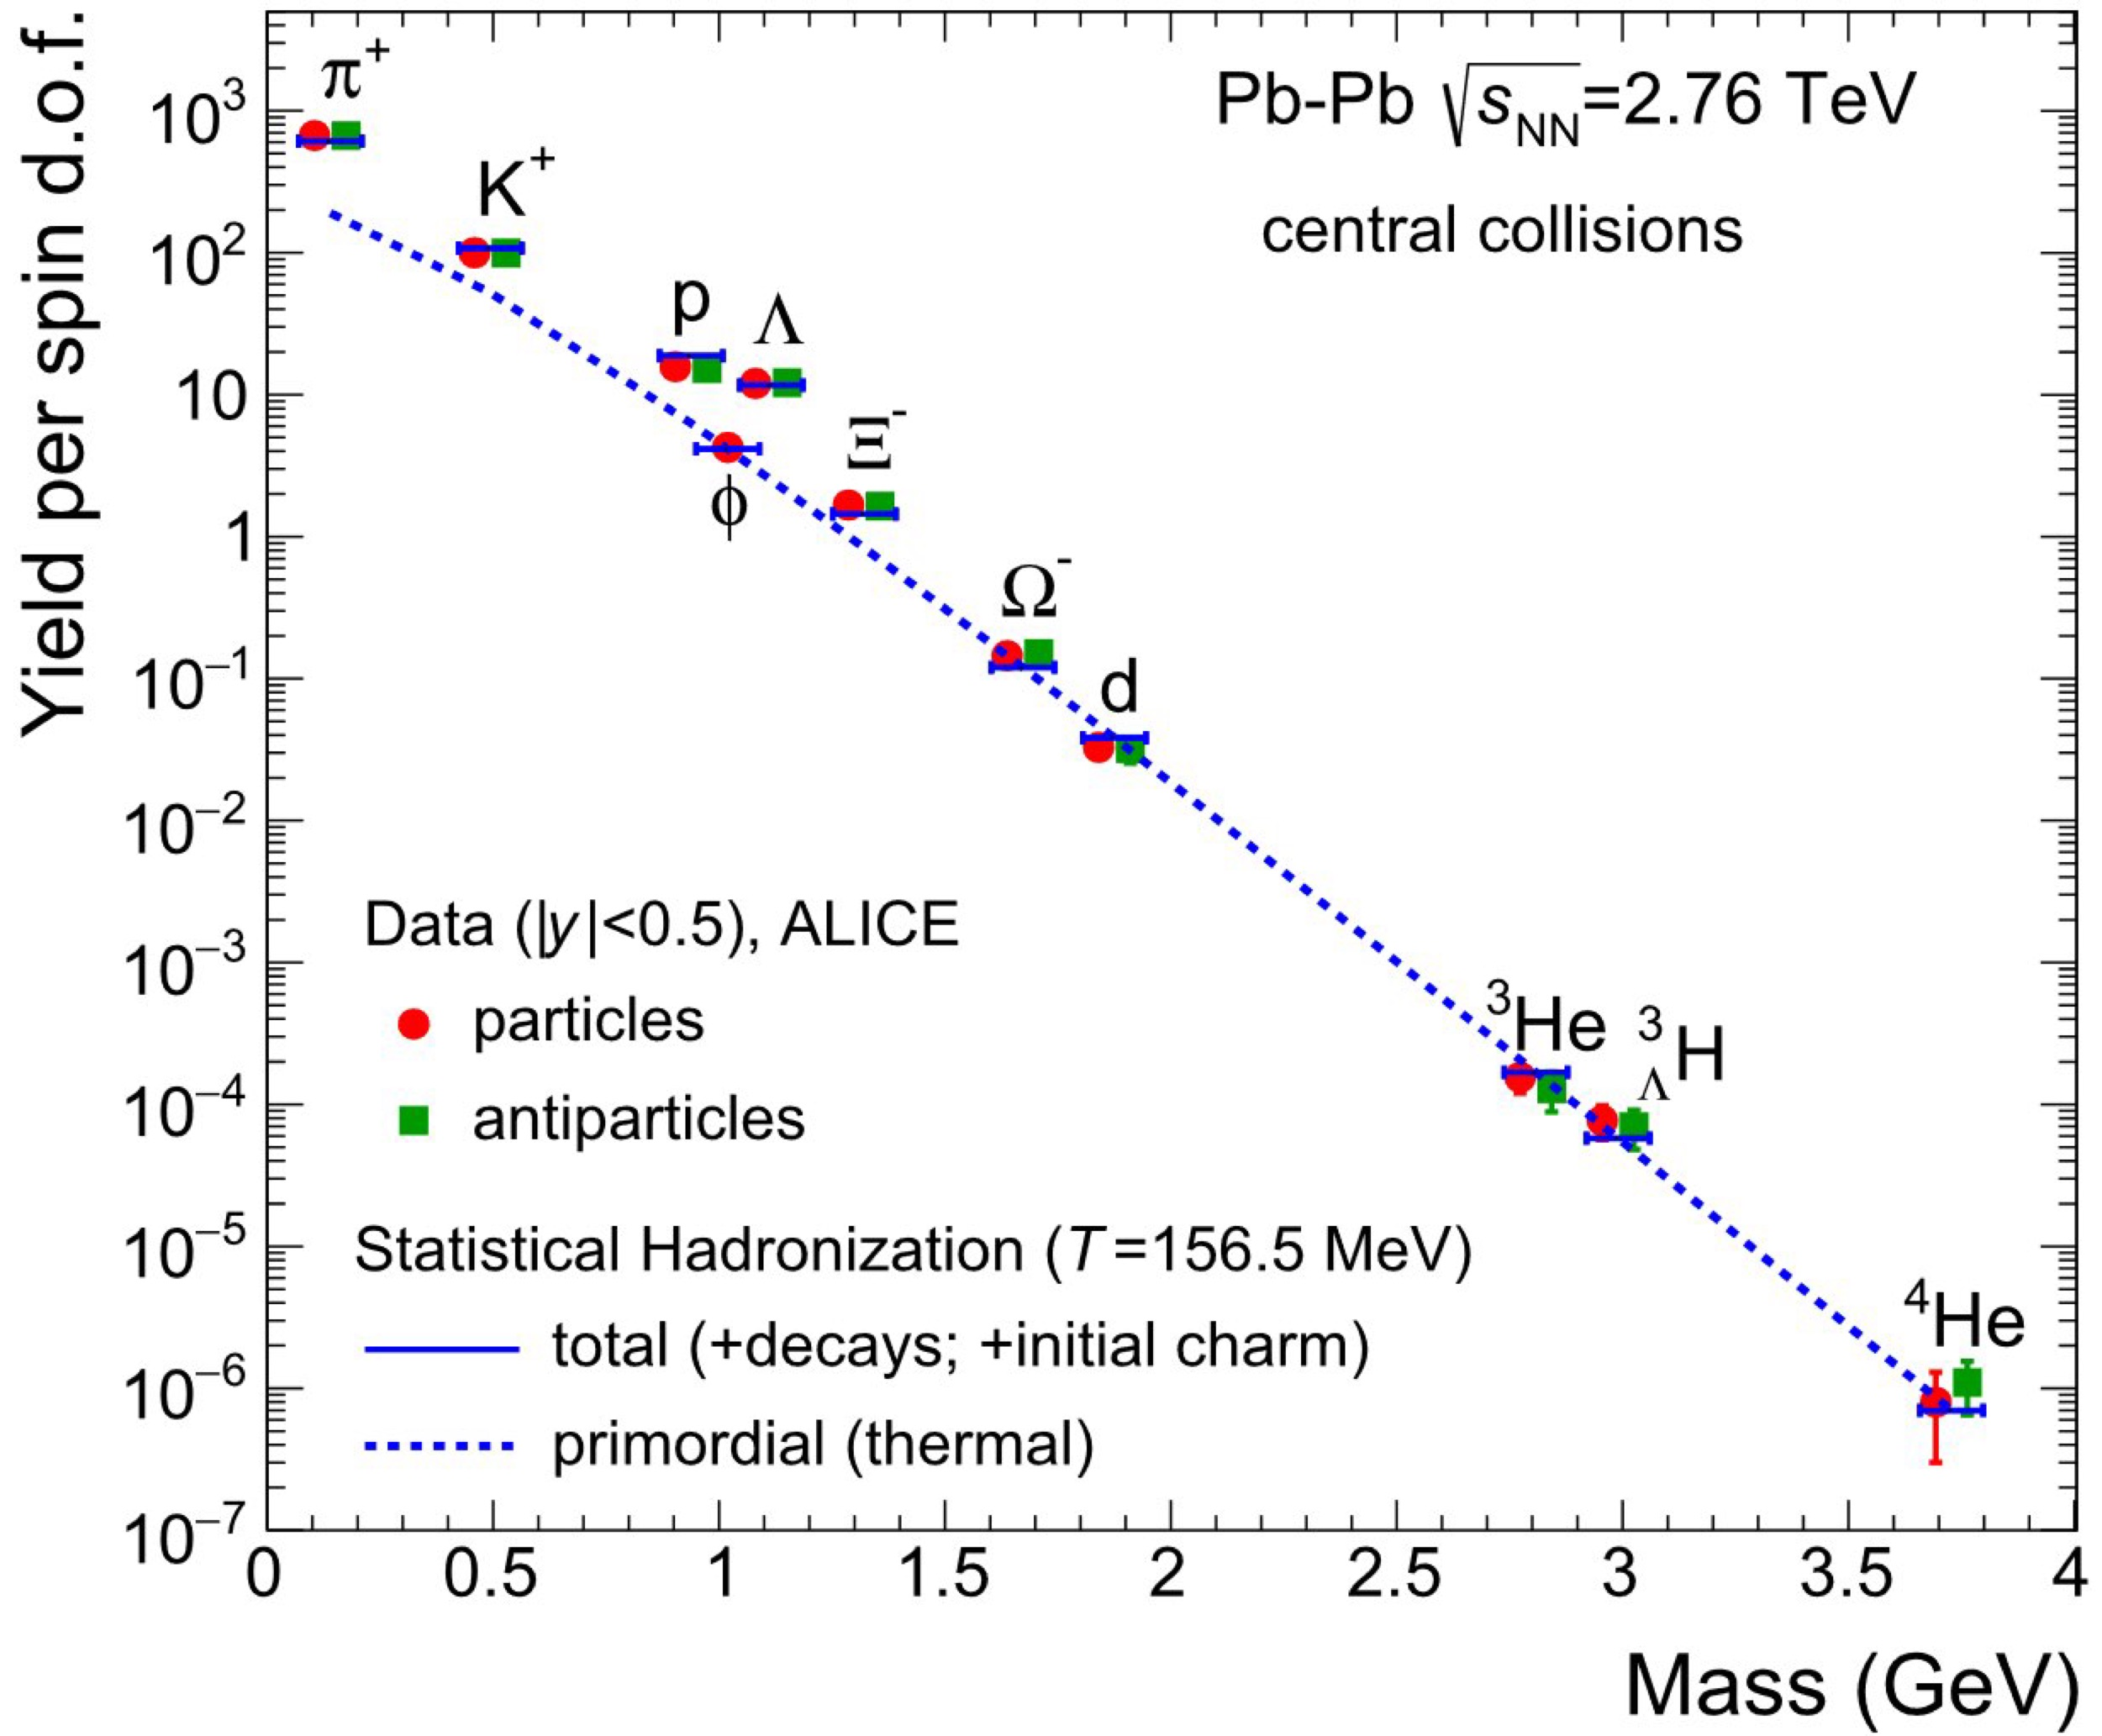
\includegraphics[width=0.6\linewidth]{image/2-modelli/mass_yield.jpg}
    \captionwithsource{(Linea tratteggiata) Variazione della produzione delle (anti)particelle rispetto alla rapidità (normalizzato  degenerazione di spin) in funzione della massa della particella, in confronto con i dati di ALICE.}{\cite{mass_yield}}
    \label{fig:mass_yield}
\end{figure}
    \item Predizioni del rapporto tra materia e antimateria in funzione dell'energia della coppia di nucleoni.
    Si può osservare come per valori piccoli dell'energia di collisione ($\sim$ 100 GeV), il potenziale barionico, una misura del rapporto materia-antimateria, assuma valori alti, per poi tendere a zero con l'aumentare dell'energia del sistema.
    Questo è compatibile con ciò che si osserva in LHC (\autoref{fig:matter_antimatter}) in cui la simmetria tra materia e antimateria è praticamente ottenuta \cite{Tawfik_2011_matter_antimatter}.
\end{itemize}
\begin{figure}[htbp]
    \centering
    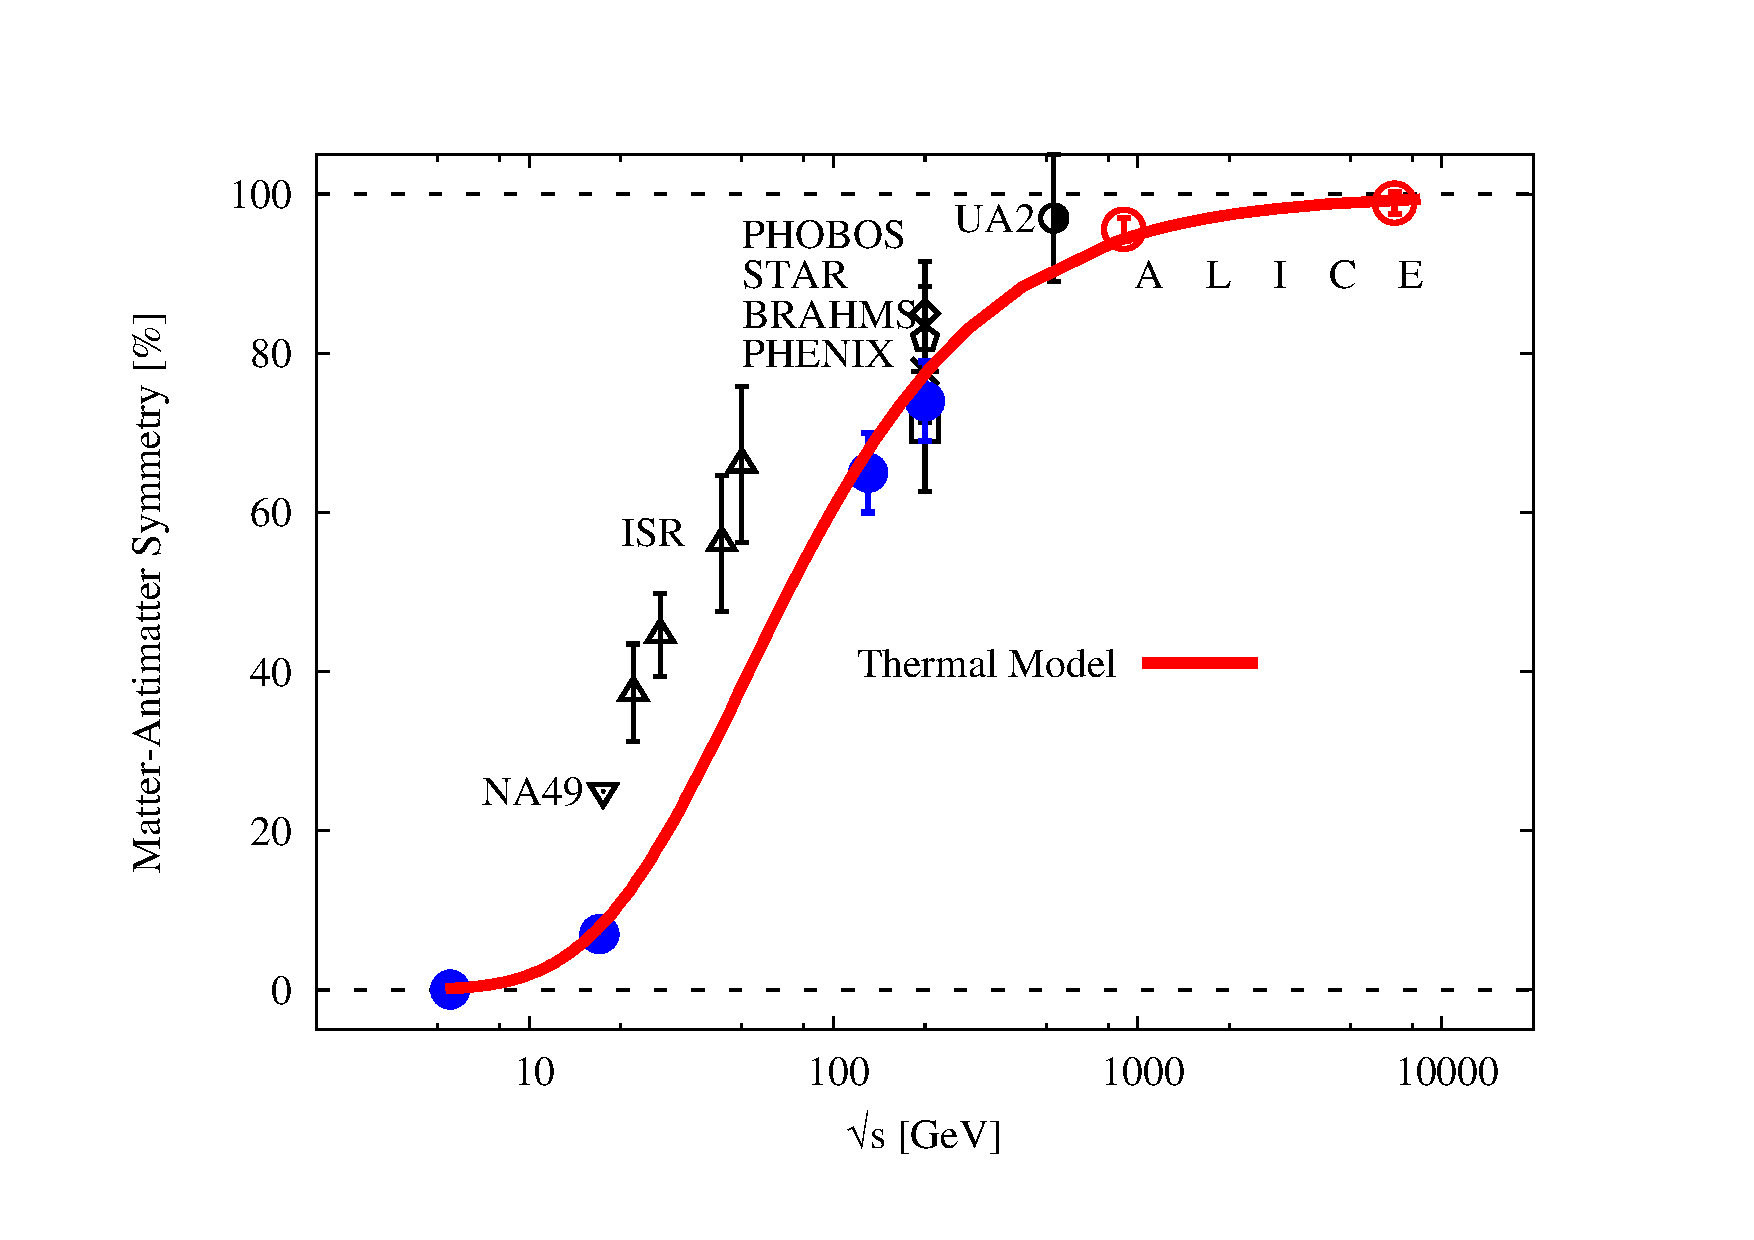
\includegraphics[width=0.8\linewidth]{image/2-modelli/antiPP_Alice2010_2.pdf}
    \captionwithsource{Rapporti di ${\bar{p}}/p$ in funzione dell'energia del centro di massa $\sqrt{s}$. I simboli vuoti indicano i risultati da vari esperimenti di collisioni pp, mentre i simboli pieni rappresentano quelli da collisioni di ioni pesanti. La curva nera rappresenta le previsioni del modello termico sul rapporto $\bar p/p$ del SMH.}{\cite{Tawfik_2011_matter_antimatter}}
    \label{fig:matter_antimatter}
\end{figure}